\section{Développement et Tests}

Après la phase de Conception, vient la phase de développement, suivie de la phase de test.

\subsection{Symfony 2}

Comme expliqué précédemment, pour ce projet, j'ai utilisé \textbf{Symfony 2}. Il s'agit d'un framework PHP suivant le pattern MVC proposant de nombreux composants pour accélérer et faciliter le développement d'une application PHP. De plus, Symfony possède une communauté très impliquée, ce qui permet de trouver de très nombreuses documentations très bien rédigées.

Symfony est sponsorisé par SensioLabs, une entreprise française. Sponsorisé car, même si cette entreprise a développé la première version du framework, elle est maintenant entretenue par la communauté, en tant que projet Open-Source (\textit{MIT License}). Il est actuellement dans sa version 2.7.

Symfony offre la possibilité d'ajouter de nombreux `` Bundles '' indépendants permettant d'ajouter des fonctionnalités adaptées à nos besoins. De plus, Symfony utilise \textbf{Composer} qui est un `` Dependency Manager '' (ou gestionnaire de dépendance en français) qui permet d'ajouter un Bundle au projet en une seule commande: \textit{composer require "genemu/form-bundle"}

Symfony propose de construire une application selon la structure suivante:

\begin{figure}[H]
\begin{lstlisting}
    - app/
        - cache/
        - config/           /* Tout les fichiers de configuration
                               avec les paramètres et les routes  */
        - logs/
        - Resources/        // Les fichiers de ressources (Templates html)
        - AppKernel.php     // Base de l'application, enregistre les bundles
        - ...

    - bin/                  // Géré par Symfony, pas toucher

    - doc/                  // La documentation de l'application

    - src/                  // La plupart de notre code est ici
        - AppBundle         // Bundle principal de l'application

            - [...]         // Plus de détails à suivre

    - vendor/               /* Ici se trouve les bundles externes */

    - web/                  /* Ici, nous trouvons tout les fichiers css,
                               js, les images, etc... Il s'agit du dossier
                               qui sera accessible aux utilisateurs      */

    - composer.json         /* Ce fichier liste tous les bundles que 
                               nous utilisons                       */
\end{lstlisting}
\caption{Architecture proposée par le framework Symfony}
\end{figure}

\subsubsection*{Les composants Symfony}

Un des composants que j'ai le plus utilisé dans Symfony est: `` HTTPFoundation ''. En effet, il gère de lui même les requêtes récupérer pour les offrir dans une classe \textbf{Request} et il est possible de créer une réponse très simplement en utilisant la classe \textbf{Response}.

\begin{figure}[H]
\begin{lstlisting}[frame=single]
<?php

[...]

use Symfony\Component\HttpFoundation\Response;
use Symfony\Component\HttpFoundation\Request;

[...]

function indexAction(Request $request) {

    $name = $request->query->get('name');

    return new Response("Hello".$name);
}
[...]

\end{lstlisting}
\caption{Code simplifié avec exemple d'HTTPFoundation}
\end{figure}

Comme on peut le voir sur les quelques lignes de code précédentes, il est facile de saluer un utilisateur nous donnant son nom. Si nous voulions faire une page privée, nous pourrions renvoyer un code \textbf{403 Forbidden} simplement en ajoutant 403 en argument du constructeur de Response.

Durant le développement d'ODE, j'ai utilisé de nombreux autres composants de Symfony: \textit{Controller}, \textit{FormBuilder}, \textit{Routing}, etc...

\vspace{1cm}

Pour revenir sur l'architecture proposée par Symfony (Figure 5), nous pouvions trouver le dossier AppBundle qui est prévu pour y déposer la majorité de notre code.

\nb{Change number figure}

Il est conseillé de mettre son code selon l'architecture suivante:

\subsubsection*{Backend}

Dans le dossier \textbf{Backend/}, j'ai déposé les quelques classes permettant de stocker et de retrouver des données dans la base données: \textit{CalDAV/Auth.php}, \textit{CalDAV/Principals.php}, \textit{CalDAV/Calendar.php} et \textit{Users/UserManager.php}.

Les trois premières classes étant liées à SabreDAV, j'en parlerai dans la section suivante. La dernière, \textbf{UserManager}, est, quant à elle, liée à \textbf{FOSUSerBundle}; il s'agit d'un bundle permettant une gestion simplifiée des utilisateurs. Il gère, entre autres, l'inscription, la connexion, le chiffrage des mots de passes, les sessions liées à l'utilisateur, les rôles, etc...

\subsubsection*{Controller}

Dans ce dossier, j'ai déposé les classes de mes Contrôleurs (\textit{sachant que Symfony respecte le design pattern MVC}).

La première classe, \textbf{DefaultController} est le contrôleur le plus léger (2 fonctions): indexAction pour afficher la page d'accueil du site et testAction qui m'a servi à écrire quelques lignes de php pour tester rapidement mon code.

La seconde classe, \textbf{CalDAVController} est le contrôleur permettant de faire le lien avec SabreDAV (plus d'explication dans la section 3.2).

La troisième, \textbf{BrowserController} est le contrôleur définissant le Front-End de l'application. Il gère les pages et les formulaires proposés à l'utilisateur. Il est notamment en lien avec FOSUserBundle pour intégrer la connexion et l'inscription des utilisateurs.

Enfin, \textbf{APIController} est le contrôleur délivrant l'API. Il s'agit là de la partie de l'application délivrant la promesse de l'\textbf{Open Data}.

\subsubsection*{Entity}

Le dossier \textbf{entity/} est celui qui contient le \textbf{modèle} de l'application.

\nb{Plus de truc}

\subsubsection*{Form}

Ce dossier permet de gérer la création des formulaires en lien avec le modèle. Pour proposer des formulaires ergonomiques, j'ai utilisé un bundle, \textbf{MopaBootstrapBundle}, qui permettait d'inclure \textbf{Bootstrap} dans l'application, notamment dans la création des champs des formulaires.

\begin{figure}[H]
\begin{center}
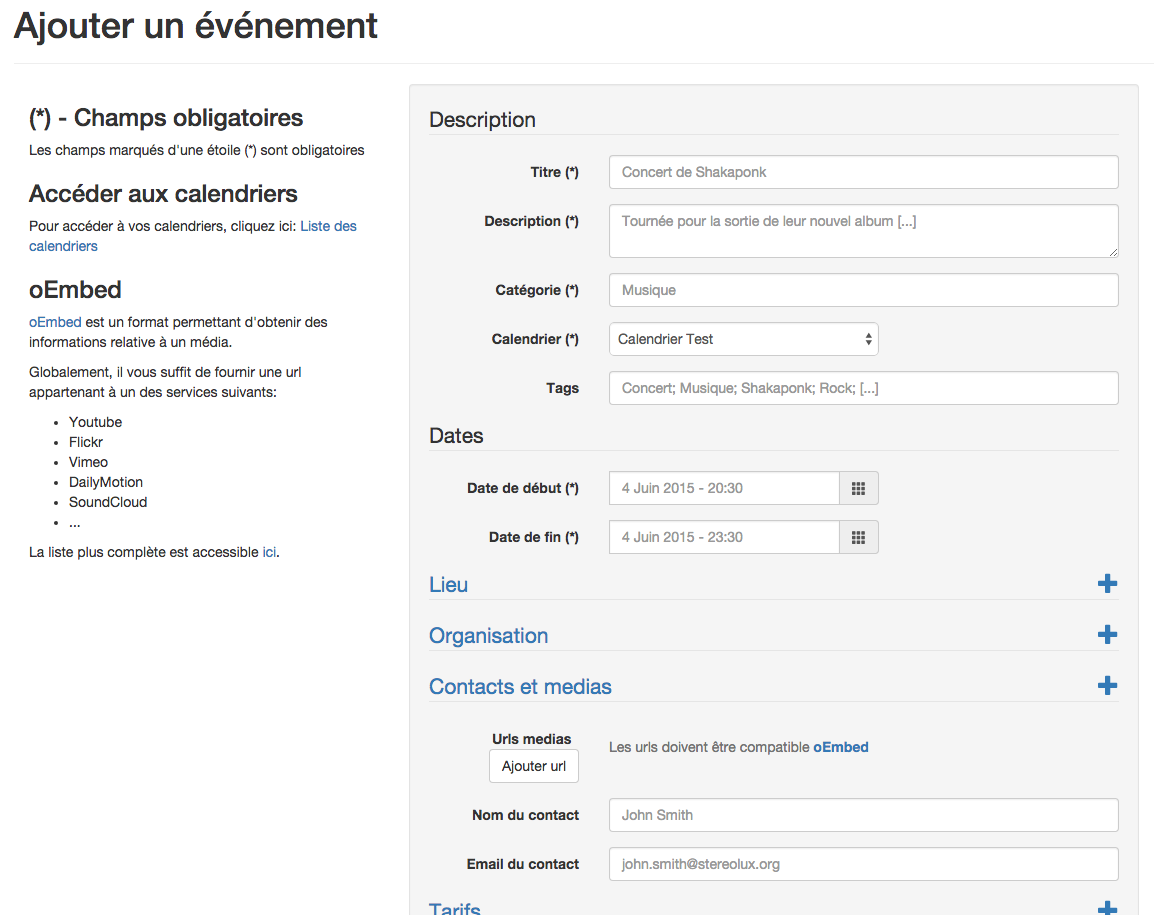
\includegraphics[height=100mm]{formulaire_event.png}
\end{center}
\caption{Formulaire de création d'un événement}
\end{figure}

\subsubsection*{Resources}

Ce dossier est en lien avec le dossier \textit{app/Resource/}. En effet, il possède aussi des fichiers de configuration, de routes, mais aussi les librairies js et css à inclure dans le dossier \textit{web/}. Pour les besoins de l'application, j'ai écrit un fichier Javascript simple pour afficher un calendrier avec une coloration sur les dates de l'événement.

\begin{figure}[H]
\begin{center}
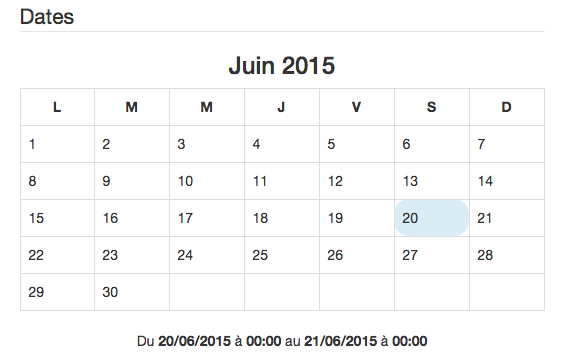
\includegraphics[height=55mm]{calendrier_js.png}
\end{center}
\caption{Calendrier généré avec javascript}
\end{figure}

\subsubsection*{Service}

Un service (dans Symfony) est un composant, un module, qui remplit une fonction et qui peut être injecté dans le conteneur de dépendance pour être rendu accessible dans toute l'application. Cette fonction peut être très simple: envoyer des e-mails, vérifier qu'un texte n'est pas un spam, etc. Un service est donc un objet PHP qui a pour vocation d'être accessible depuis n'importe où dans le code. Pour chaque fonctionnalité dont je peux avoir besoin dans mon application, je peux créer un ou plusieurs services.

Symfony utilise un `` ServiceContainer '' qui enregistre tout les services. Il est ainsi possible d'accèder aux services depuis les contrôleurs facilement:

\begin{figure}[H]
\begin{lstlisting}[frame=single]
<?php

[...]

function indexAction(Request $request) {

    $slug = $this->get('slugify')->slugify("ExEmplE èéàó à");

    return new Response($slug);

    /* Le code précédent renverra la chaine de caractère suivante:
       exemple-eeao-a
    */
}
[...]

\end{lstlisting}
\caption{Code simplifié avec exemple d'un Service}
\end{figure}

Le code précédent est une démonstration de l'appel au service \textbf{Slugify}, permettant de générer des slug `` URL Friendly ''.

\subsection{Intégration de SabreDAV}

Après avoir décidé d'utiliser le protocol CalDAV pour le projet, j'ai cherché une librairie PHP permettant d'implémenter CalDAV dans Symfony. Malheureusement, il n'existe pas de Bundle tout prêt pour cette utilisation. Cependant, durant ma recherche, j'ai découvert \textbf{SabreDAV}. Il s'agit d'un serveur php capable de gérer les rêquetes ``PROPPATCH'', ``MKCALENDAR'', etc. propres à CalDAV.

SabreDAV est un projet Open Source développé par Fruux. Fruux est une entreprise éditrice qui fait partie du \textbf{Calendaring and Scheduling Consortium}, discutant sur le standard CalDAV, au côté d'Apple, Google, IBM et d'autres.

SabreDAV possède sa propre architecture, il a donc fallu l'intégrer dans l'application. Pour cela, j'ai créé un Contrôleur spécialement pour la partie CalDAV (CalDAVController.php). Au niveau des routes, j'ai les ai toutes redirigées vers la méthode `` indexAction '' du contrôleur. Ainsi, j'ai pu transmettre la requête directement au système de SabreDAV.

Le problème que j'ai rencontré par la suite était le fait que SabreDAV gérait lui-même la constuction et l'envoi de la réponse, ce qui perturbait le fonctionnement de Symfony.

Grâce à de nombreuses recherches sur le sujet, j'ai découvert que Symfony proposait une classe, \textbf{StreamedResponse}, permettant de gérer ce cas de figure. En effet, StreamedResponse prend en argument une fonction de callback dans laquelle la réponse envoyée par SabreDAV sera attrapée par Symfony puis renvoyée vers l'utilisateur. Cela permet aussi de logger les messages renvoyés, ce qui m'a été très utile tout au long du développement de l'application.

\begin{figure}[H]
\begin{lstlisting}[frame=single]
<?php

[...]

    public function indexAction(Request $request)
    {
        [...]

        $server = new CalDAVServer();

        $callback = function () use ($server, $request) {

            [...]

            $server->exec();

            /* These two lines log the request and the response */
            $responseBody = $server->httpResponse->getBodyAsString();
            $this->logIt($request, $server->httpResponse, $responseBody);
        };

        return new StreamedResponse($callback);
    }
[...]

\end{lstlisting}
\caption{Code simplifié avec exemple de StreamedResponse}
\end{figure}

Niveau Backend, SabreDAV a été conçu pour laisser le choix aux utilisateurs. En effet, la librairie utilise des interfaces pour les classes de Backend, ainsi, j'ai pu implémenter moi même les classes, d'abord avec ElasticSearch, puis avec PostgreSQL.

Les trois classes de Backend que j'ai implémentées sont les suivantes:

\textbf{Auth.php}: Celle-ci permet d'authentifier l'utilisateur se connectant depuis un client compatible CalDAV.

\textbf{Principals.php}: Cette classe permet de gérer l'accès, la création et la suppression des `` Principals ''. Il s'agit d'un concept propre à CalDAV, que l'on pourrait résumer par un dossier pour gérer les différents calendriers.

\textbf{Calendar.php}: C'est la classe la plus importante du Backend. En effet, elle rassemble toutes les fonctions pour créer, récupérer, modifier et supprimer un calendrier ou un événement. Elle s'occupe aussi des souscriptions et de lister les calendriers présents sur le serveur. J'utilise cette classe de nombreuses fois dans les contrôleurs, car même si elle est utilisée par SabreDAV, elle s'adapte très facilement à n'importe quelle utilisation.

\subsection{Implémentation avec ElasticSearch}

\textbf{ElasticSearch} est un moteur d'indexation et de recherche. Les principaux atouts d'ElasticSearch sont sa capacité à stocker les données sous le format JSON, ainsi que sa capacité à offrir de nombreux graphiques et statistiques sur l'utilisation du service.

ElasticSearch se base sur Apache Lucene, il est donc propulsé par Java. L'installation d'ElasticSeach requiert de plus la version 1.8 de la Java Virtual Machine. ElasticSearch n'étant pas adapté à OSX, j'ai dû installer une machine virtuelle sur mon Mac. Pour cela, j'ai utilisé \textbf{Vagrant}.

\textbf{Vagrant} est un outil permettant de gérer des machines virtuelles simplement. Il utilise lui même le logiciel très connu: \textbf{VirtualBox}. Pour configurer la machine virtuelle, il suffit de modifier un fichier de configuration simple.

Après avoir installé Vagrant, il suffit d'éxécuter les commandes suivantes:

\begin{lstlisting}
vagrant init hashicorp/precise32
vagrant up
vagrant ssh
\end{lstlisting}

Et on se retrouve dans une machine virtuelle avec Ubuntu 14.04.

En ce qui concerne l'installation d'ElasticSearch sur la machine virtuelle, j'ai produit la \blurl{https://github.com/LiberTIC/ODEV2/blob/77e78f9cc36d0bc5c22eadbf2e39ab2959f10c45/doc/Elasticsearch_install.md}{Documentation de l'installation} sur le Github pour que d'autres puissent le refaire facilement.

Pour faire le lien entre Symfony et le serveur ElasticSearch, j'ai créé la classe ESManager permettant de faire des requêtes de façon simple depuis les contrôleurs. De plus, je l'ai ajouté au ServiceContainer de Symfony pour l'utiliser facilement.

Un des problèmes rencontrés avec ElasticSearch est le fait qu'ElasticSearch est fait pour l'indexation de données, mais il ne donne pas suffisamment de garantie en tant que moteur de persistence de données.

Un autre problème venait l'utilisation que j'en ai fait: le stockage complet des données, posait des problèmes notamment pour l'indexation du jCal d'un événement.

En effet, ElasticSearch se décrit comme `` SchemaLess ''. Cela veut dire que quel que soit le \textbf{document} (\textit{structure JSON}) que nous allons \textbf{indexer}, ElasticSearch va produire un document de \textbf{Mapping} qui décrit le Schema du document que nous venons de lui donner sous la forme: `` Nom => Type ''. Il s'agit là d'une fonctionnalité très appréciée dans l'utilisation d'ElasticSearch dans la plupart des cas. Cependant, jCal suit une architecture différente de JSON comme le montre la figure suivante, et je devais donc modifier la façon dont je stockais le jCal pour l'adapter à ElasticSearch.

\begin{figure}[H]
\begin{lstlisting}[frame=single]

// JSON Classique

{
    "glossary": {
        "title": "example glossary",
        "GlossDiv": {
            "title": "S",
            "GlossList": {
                "GlossEntry": {
                    "ID": "SGML",
                    "SortAs": "SGML",
                    "GlossTerm": "Standard Generalized Markup Language",
                    "Acronym": "SGML",

[...]

\end{lstlisting}
\caption{Exemple JSON}
\end{figure}
\begin{figure}[H]
\begin{lstlisting}[frame=single]

// jCal

["vevent",
         [
           ["dtstamp", {}, "date-time", "2006-02-06T00:11:21Z"],
           ["dtstart",
             { "tzid": "US/Eastern" },
             "date-time",
             "2006-01-02T12:00:00"
           ],
           ["duration", {}, "duration", "PT1H"],
           ["rrule", {}, "recur", { "freq": "DAILY", "count": 5 } ],
           ["rdate",
             { "tzid": "US/Eastern" },
             "period",
             "2006-01-02T15:00:00/PT2H"
           ],
           ["summary", {}, "text", "Event #2"],
           ["description",

[...]

\end{lstlisting}
\caption{Exemple jCal}
\end{figure}

\newpage

\subsection{Implémentation avec PostgreSQL}

Finalement, durant une réunion hebdomadaire, je me suis rendu compte que le projet avait légèrement évolué en ce qui concerne son utilisation. En effet, la façon dont j'avais conçu ODE était la suivante: Une instance unique du projet avec un grand nombre de données. Or, petit à petit, ODE s'adaptait mieux au format: Un grand nombre de petites instances du projet.

J'ai donc ré-évalué la question du stockage des données, et je me suis rendu compte qu'ElasticSearch, bien qu'adapté pour l'instance unique, n'étais pas du tout adapté pour la façon dont nous envisagions ODE à ce moment. Ainsi, j'ai décidé, avec l'accord de mon maître de stage, de remplacer l'utilisation d'ElasticSearch pour le remplacer par une base de données PostgreSQL.

À partir de là, j'ai ré-implémenté les classes d'implémentation du BackEnd SabreDAV pour les adapter à PostgreSQL.

Pour communiquer entre l'application et PostgreSQL, j'ai utilisé \textbf{Pomm}. Il s'agit d'un framework open source d'accès à la base de données lié avec un Object Model Manager dédié à PostgreSQL. Il offre une approche alternative à ORM pour l'utilisation des bases de données dans le développement web. Pomm est développé par Grégoire Hubert sous licence Creative Commons BY-SA.

À l'instar de la création d'un service ESManager pour utiliser facilement ElasticSearch, j'ai créé le service PommManager possédant des fonctions telles que: createOne, deleteOne, findOne, findById, etc.

Le problème principal de mon utilisation de PostgreSQL fut le manque du module PostgreSQL de PHP natif sur OSX. Cependant, je n'ai pas rencontré d'autre problème particulier.

\subsection{Fondation d'une API REST}

Créer une API \textbf{REST} n'est pas simple. En effet, il ne s'agit ni d'un standard, ni d'un protocole. C'est pourquoi je me suis longuement documenté sur les principes de REST, sur ses bonnes pratiques, mais aussi sur ses limites. \rf{restsymfony}\rf{hateoas}\rf{restandhateoas}

Un des points à savoir, est la progression constante de la part d'API JSON face aux API XML, comme le montre la figure suivante:

\begin{figure}[H]
\begin{center}
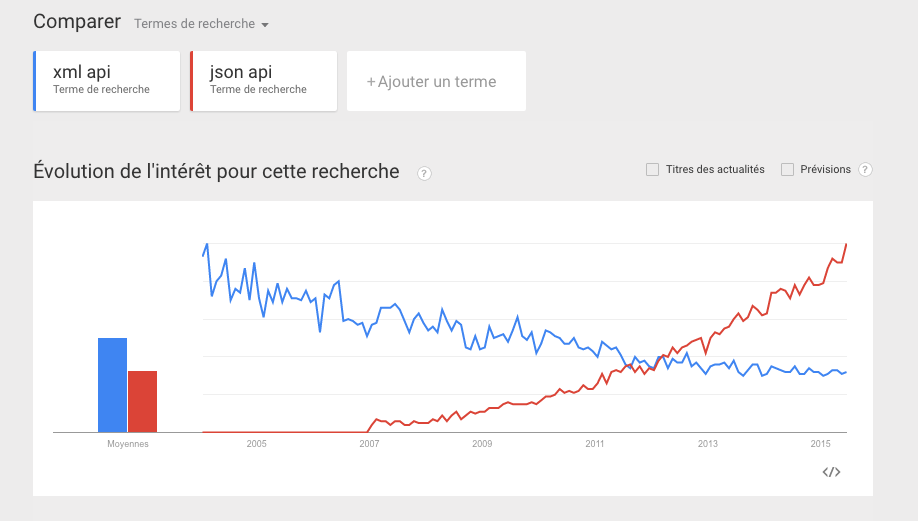
\includegraphics[height=70mm]{xml-vs-json.png}
\end{center}
\caption{Graphique de recherche des termes XML API et JSON API}
\end{figure}

\textit{Source: \blurl{http://ur1.ca/ey5o6}{Google Trends}}

Durant cette recherche, j'ai découvert la notion de HATEOAS \textit{(Hypermedia As The Engine Of Application State)}. Il s'agit d'un concept d'architecture de l'application pour rendre l'API `` Explorable '', c'est-à-dire qu'il est possible de se déplacer dans l'API avec des `` liens '' pour découvrir les opérations disponibles.

HATEOAS est décrit dans le Modèle de Maturité de Richardson \rf{richardson} comme étant le troisième niveau de maturité d'une application REST, les deux premiers étant les Ressources et les Verbes HTTP. Il apporte une dimension sémantique aux API.

\begin{figure}[H]
\begin{center}
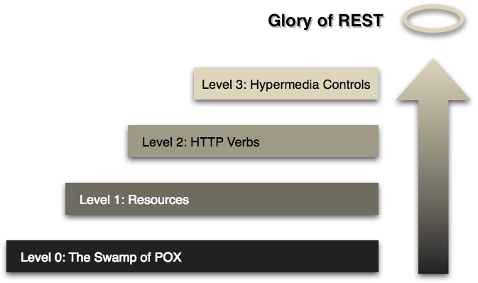
\includegraphics[height=70mm]{richardson_maturity_model.png}
\end{center}
\caption{Graphique de recherche des termes XML API et JSON API}
\end{figure}

Sachant qu'une des composantes principales de ce projet est l'Open Data, l'API REST doit permettre de fournir toutes les données de l'application.

J'ai documenté toutes les opérations possibles de l'API sur Github à l'adresse suivante: \url{https://github.com/LiberTIC/ODEV2/blob/master/doc/RestAPI.md}.

J'ai essayé de retourner le plus souvent les bons codes de status HTTP. \textit{(Même si je n'ai pas réussi à mettre le 418 - I'm a teapot...)}

\subsection{Tests unitaires}

Comme pour toutes applications, il est important d'effectuer des tests pour s'assurer de la fiabilité de notre code. Symfony 2 intègre un composant de Tests, c'est donc facile d'écrire les tests unitaires pour l'application.

\begin{figure}[H]
\begin{lstlisting}[frame=single]
<?php

namespace AppBundle\Tests\Controller;

use Symfony\Bundle\FrameworkBundle\Test\WebTestCase;

class DefaultControllerTest extends WebTestCase
{
    public function testIndex()
    {
        $client = static::createClient();

        $crawler = $client->request('GET', '/app/example');

        $this->assertEquals(200, $client->getResponse()->getStatusCode());
        $this->assertTrue(
            $crawler->filter('html:contains("Homepage")')->count() > 0);
    }
}

\end{lstlisting}
\caption{Code simplifié de Test avec Symfony}
\end{figure}

Cependant, à cause de la courte durée de mon stage, je n'ai pas pu écrire la plupart des tests unitaires de l'application.

\subsection{Tests de comportement}

À l'instar des tests unitaires, je n'ai pas pu effectuer des tests de comportement. Cependant, je les ai préparé grâce à Behat. Pour cela, j'ai écrit des fichiers de `` Scénarios '' pour décrire le comportement attendu de mon application.

\begin{figure}[H]
\begin{center}
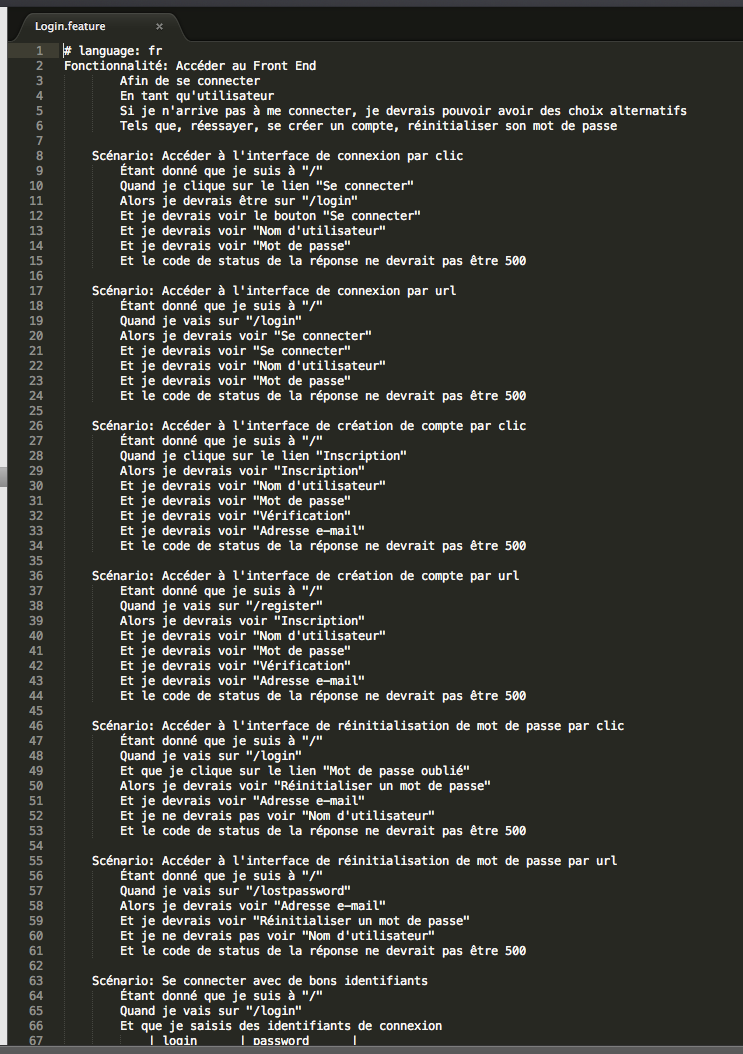
\includegraphics[height=140mm]{login_feature.png}
\end{center}
\caption{Scénarios de login sur l'application}
\end{figure}

L'avantage de Behat est de pouvoir écrire les scénarios en Français, pour pouvoir discuter des comportements attendu plus facilement avec les collaborateurs. En effet, il est possible de définir de nouvelles méthodes du Context pour créer de nouvelles phrases, adaptées à notre application.